\section{流化床反应器}


\begin{frame}
    \frametitle{流态化}
    当流体自下而上地流过颗粒物料层时，随着流速的增加，流体的压力降将发生变化。

        \begin{minipage}{0.5\linewidth}
            \begin{itemize}
                \item 在低流速范围内，压力降随着流速的增大而增加，床层内的颗粒处于静止状态，属于固定床范围。
                \item 但当流速增大到与一定值时，再加大流速，颗粒则处于运动状态，在相当宽的流速范围内，压力降几乎保持为一定值。
            \end{itemize}
        \end{minipage}\hfill
        \begin{minipage}{0.46\linewidth}
            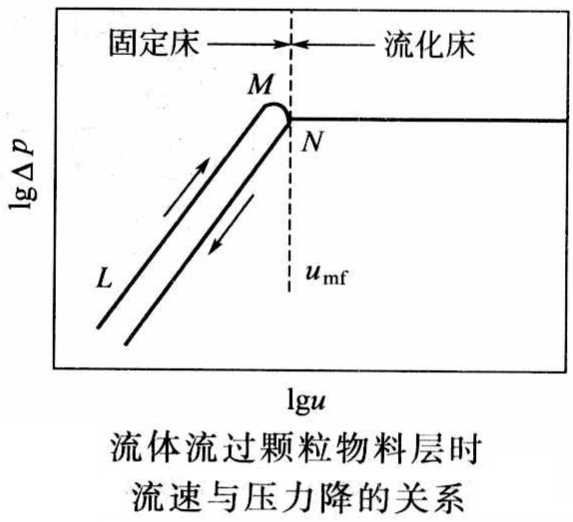
\includegraphics[width=\linewidth]{figures/fig7.10.png}
        \end{minipage}

\end{frame}


\begin{frame}
    \frametitle{最小流化速度}
    颗粒处于运动状态而容器内床层又具有明显的界面，称为\highlight{流化床}。此时固体颗粒具有像流体一样的流动性质，故称\highlight{流态化}。

    点N称为临界流化点，所对应的流速叫做最小流化速度$u_\mathrm{mf}$。

    流化床的压力降可按下式计算
    \[
        \Delta p = L_\mathrm{mf}(1- \varepsilon_\mathrm{mf})(\rho_\mathrm{s} - \rho_\mathrm{f})g
    \]
    $L_\mathrm{mf}$和$\varepsilon_\mathrm{mf}$为床层颗粒开始流化时的床层高度和空隙率，$\rho_\mathrm{s}$及$\rho_\mathrm{f}$则分别为固体和流体的密度。

    由于临界流化点为固定床与流化床的交界点，
    \[
        \Delta p=f \frac{L_\mathrm{mf} u_\mathrm{mf}^{2} \rho(1-\varepsilon_\mathrm{mf})}{d_{\mathrm{s}} \varepsilon^{3}}
    \]
    两式联立可求解$u_\mathrm{mf}$。

\end{frame}


\begin{frame}
    \frametitle{流态化}

    流化介质的密度与固体颗粒的密度相差越大，所形成的流化床越不均匀。
    \begin{itemize}
        \item 用液体将颗粒流化，称为散式流化，颗粒在床层中分散得较均匀。
        \item 用气体作流化介质时，属于不均匀流化或称聚式流化。
    \end{itemize}

    也可按弗鲁特数$Fr = u^2/gd_\mathrm{p}$的大小来划分
    \begin{itemize}
        \item $Fr<1$为均匀流化，
        \item $Fr>1$则为不均匀流化或聚式流化。
    \end{itemize}

\end{frame}


\begin{frame}
    \frametitle{气固流化床}
    在气固流化床中，气速大于临界流化速度时，部分气体以气泡的形式通过床层，犹如气体成泡状通过液体层一样。
    \begin{figure}[htpb]
        \centering
        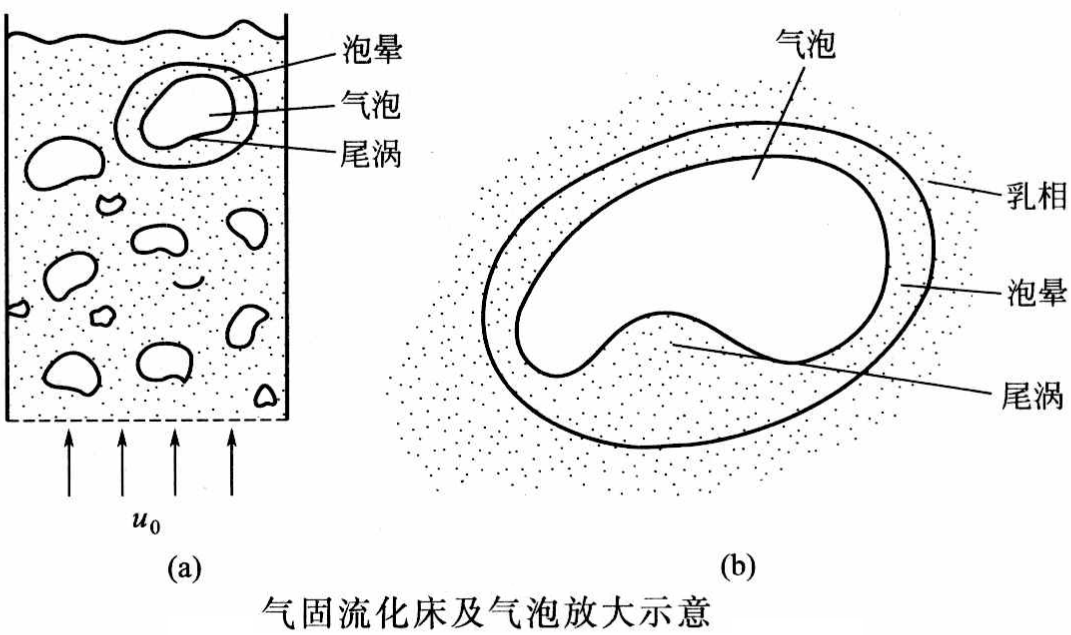
\includegraphics[width=.5\linewidth]{figures/fig7.11.png}
    \end{figure}
    由于床层内气体和颗粒的剧烈运动，使床层内温度均匀，这是流化床的一个主要特点。流化床传热效果也要优于固定床，传数系数比后者大得多。

\end{frame}


\begin{frame}
    \frametitle{流化床催化反应器}

        \begin{minipage}{0.13\linewidth}
            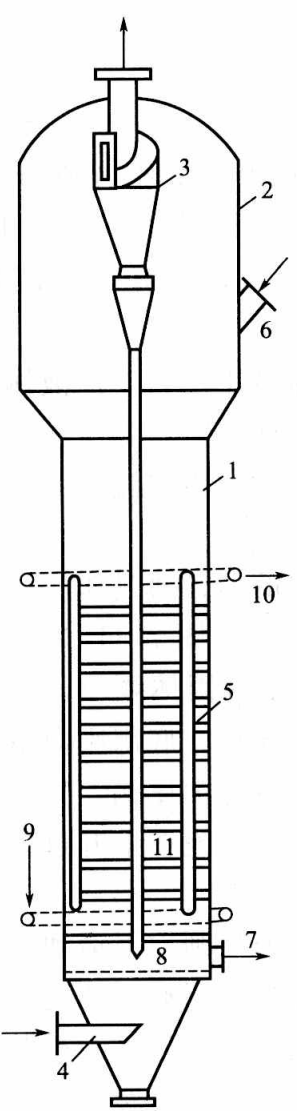
\includegraphics[width=\linewidth]{figures/fig7.12.png}
        \end{minipage}\hfill
        \begin{minipage}{0.2\linewidth}
            \scriptsize{\begin{enumerate}
                \item 壳体
                \item 扩大管
                \item 旋风分离器
                \item 流化气体入口
                \item 换热管
                \item 催化剂入口
                \item 催化剂出口
                \item 气体分布板
                \item 冷却水进口
                \item 冷却水出口
                \item 分布板
            \end{enumerate}}
        \end{minipage}\hfill
        \begin{minipage}{0.64\linewidth}
            \begin{itemize}
                \item 反应气体从进气管4进入反应器
                \item 经气体分布板8进入床层
                \item 设置内部构件（挡板11）打碎气泡，改善气固接触和减小返混
                \item 换热装置，可以将换热器装在床层内，也可以在床层周围装设夹套，视热负荷大小而定。
                \item 催化剂颗粒从进口6加入，由出口7排出。
                \item 扩大段，使气流速度降低，从而部分较大的颗粒可以沉降下来，落回床层中去。较细的
                颗粒则通过反应器上部的旋风分离器3分离出来返回床层。反应后的气体由顶部排出。
            \end{itemize}
        \end{minipage}

\end{frame}


\begin{frame}
    \frametitle{流化床催化反应器}

        \begin{minipage}{0.28\linewidth}
            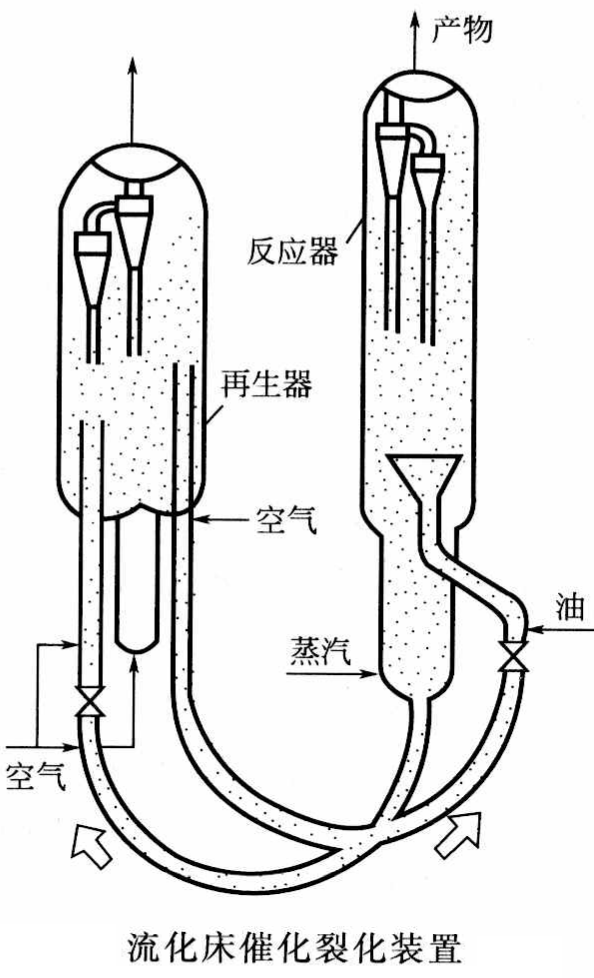
\includegraphics[width=\linewidth]{figures/fig7.13.png}
        \end{minipage}\hfill
        \begin{minipage}{0.68\linewidth}
            实际生产中，有些催化反应过程所使用的催化剂很快就失活，需要连续进行再生。

            石油炼制工业中将重质油进行催化裂化以获得更多的轻油 ， 正是采用了流化床反应器而取得突破性的成果。

            裂化反应同时还发生结焦反应，焦沉积在催化剂表面上而降低其催化活性，因此需要再生。再生的方法是用空气将沉积在催化剂上的焦燃烧，使其活性恢复。

            再生器中进行烧焦反应，放热。

            反应器中进行裂化反应，吸热。

        \end{minipage}

\end{frame}


\begin{frame}
    \frametitle{循环流化床反应器}

        \begin{minipage}{0.22\linewidth}
            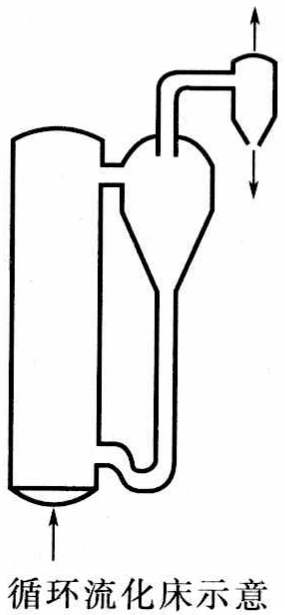
\includegraphics[width=\linewidth]{figures/fig7.14.png}
        \end{minipage}\hfill
        \begin{minipage}{0.76\linewidth}
            
            \begin{itemize}
                \item 低速流化床，固体颗粒不被气体带出，颗粒在反应器内循环，类似于液体沸腾，故亦称为沸腾床。
                \item 近年来随着流态化技术的发展，流化床倾向在高气速下操作，此时气速大于固体颗粒的带出速度，固体颗粒被带出经分离后再循环进入反应器，这种称为循环流化床，亦称快速流化床。
                \item 循环流化床中气固间相对速度即滑落速度大，使床内保持较高固相浓度，大大强化了气固间的传热与传质。
            \end{itemize}
        \end{minipage}

\end{frame}


\begin{frame}
    \frametitle{流化床催化反应器的特点}
    \cbf{优点}
    \begin{itemize}
        \item[\bigcirc] 可以使用小粒度的催化剂，因而内扩散的影响完全可以忽略，提高了催化剂的利用率。
        \item[\bigcirc] 温度均匀，完全可以实现等温操作，这对于某些反应温度范围要求很窄的催化反应过程十分合宜。
        \item[\bigcirc] 流化床反应器催化剂的加入和卸出都十分方便，非常适合催化剂需要连续再生的反应。
        \item[\bigcirc] 压力降不随气速而变化。
    \end{itemize}
    \cbf{缺点}
    \begin{itemize}
        \item[\times] 由于磨损和气体带走而造成催化剂损失大，这点对于贵金属催化剂是难以承受的；
        \item[\times] 返混严重；
        \item[\times] 气体以气泡形式通过床层而造成气固接触不良。
    \end{itemize}
\end{frame}